\documentclass[12pt,a4paper]{article}

\usepackage[utf8]{inputenc}
\usepackage[english]{babel}
\usepackage{amsmath}
\usepackage{amsfonts}
\usepackage{amssymb}
\usepackage[left=2cm,right=2cm,top=2cm,bottom=2cm]{geometry}
\usepackage{graphicx}
\usepackage{pdfpages}
\usepackage{lscape}
\usepackage{fancyhdr}

\pagestyle{fancy}
\fancyhead[L]{Josep Maria Serra Moncunill}
\fancyhead[R]{Project Charter}
\fancyfoot[C]{\thepage}

%---Begining of the Project Charter---
\begin{document}

\begin{titlepage}
\vspace*{50pt}
\begin{center}
\includegraphics[scale=0.3]{./Media/logo_ESEIAAT.jpg}\end{center}
\vspace{25pt}
\begin{LARGE}\begin{center}\textbf{Study for the computational resolution of conservation equations of mass, momentum and energy. Possible application to different aeronautical and industrial engineering problems: Case 5D}\end{center}\end{LARGE}
\vspace{15pt}
\begin{LARGE}\begin{center}Project Charter\end{center}\end{LARGE}
\vspace{40pt}
\begin{center}{\large Author: Josep Maria Serra Moncunill}\end{center}
\vspace{25pt}
\begin{center}{\large Director: Asensio Oliva Llena}\end{center}
\begin{center}{\large Co-Director: Carlos David Pérez Segarra}\end{center}
\vspace{40pt}
\begin{center}{\normalsize Delivery Date: 10th June 2017}\end{center}
\end{titlepage}

\tableofcontents
\pagebreak

%--Section 1: Aim--
\section{Aim}
The main objective of this study is to acquire a deeper understanding of the conservation equations of mass, momentum and energy, and to solve a variety of different problems involving heat transfer and fluid dynamics using numerical methods. A self-made code in C++ language will be created in order to solve these problems, and a verification of the results will be done comparing them with an analytical solution.\\
\\
Additionally, a particular case in an industrial or aeronautical application will be selected, and a code will be developed in order to solve this case. Verification of the results and optimization of the parameters will be done.

%--Section 2: Scope--
\section{Scope}
The scope of this study is stated as follows:
\begin{itemize}
\item Review of the history and evolution of computational methods and techniques involving fluid dynamics and heat transfer (State-of-the art).
\item Introduction to the finite volumes methods as well as the mathematical knowledge required for solving the conservation equations.
\item Study of the equations of heat conduction in solids, laminar convection in unsteady conditions and radiation. If there is enough time, turbulent flow will be studied as well. 
\item Development of software using C++ language capable of solving benchmark problems such as the Smith-Hutton problem or the Lid Driven Cavity.
\item Validation and verification of the codes, as well as an analysis of convergence.
\item Study of a case in a particular field of interest and discussion on the results.
\item Optimization of the code.
\end{itemize}

%--Section 3:--Requirements--
\section{Requirements}
The requirements of the study are listed below:
\begin{itemize}
\item The programming language used will be C++.
\item Codes must be designed to be executed by a personal computer.
\item Codes must be in a single file and compile with no errors.
\item Codes must run without any input parameter.
\item The mathematical method used by the codes must be Finite Volumes method.
\item Codes must be tested using benchmark cases.
\end{itemize}

%--Section 4: Background--
\section{Background}
It is well known that transfer of heat and mass, fluid flow, chemical reactions, and other related processes play a vital role in the world. These processes can be observed in an infinite number of situations. Almost all methods of power production require fluid flow and heat transfer. The same can be said about heating and cooling in buildings. Thermo-fluid processes are present in ovens, furnaces, heat exchangers, reactors and condensers. Aircrafts and automobiles require a fluid flow and heat exchange in order to function. In electrical and electronic components, heat transfer is a very important issue. Storms and fires are also caused by heat and mass transfer. Even the human body is under a process of continuous flow of heat and mass.\\
\\
Knowing the great importance of these factors in the world, it is no wonder that an accurate understanding of these processes is needed, as well as an efficient way to predict them. However, although this processes can be fully understood and expressed in a set of mathematical equations, the so called conservation equations, the nature of this processes often leads to very non-linear coupled equations and a general solution is impossible to obtain. These equations are: conservation of mass (one time dependant equation), conservation of momentum (three time dependant equations, one for each direction), and conservation of energy (one time dependant equation), often called Navier-Stokes equations. At this point, two options are possible in order to obtain the solution of these equations for a given problem: experimental tests or theoretical resolution.\\
\\
Experimental investigation using full-scale tests allow scientists con predict how identical processes will react to the same characteristics. However, these kind of tests are very expensive and, therefore, small-scale models must be used. In the process of going from a full-scale model to a small-scale one, some characteristics of the full-scale problem must be extrapolated, and the same happens with the results obtained in the small-scale one. Additionally, some features must be omitted. It should also be taken into account that results depend of the instrument precision and the discrete number of sensors used. These problems reduce the usefulness of experimental results.\\
\\
Theoretical resolution implies the resolution in all the domain of a system of non-linear coupled equations, which nowadays has resulted to be impossible. Therefore, simplifications must be made in order to obtain a solution, such as incompressibility or steady conditions. Even with simplifications, only a small fraction of problems can be solved, and with further simplifications, the more problems can be solver, but the less exact becomes the solution. In some cases, the least simplified solutions that is able to solve the problem is too simplified to obtain an exact solution.\\
\\
At this point is where numerical methods become relevant. The basics of computational fluid dynamics (CFD) consist in discretizing the domain in a finite number of zones. Inside these regions, conservation equations are linearized. This turns a system of a few non-linear equations impossible to solve into a large system of linear equations that can be solved. Although this new system of equations gives an approximated solution, with enough discretization is possible to obtain a solution with enough accuracy. However, it must be noted that since the size of the discretization depends of the performance of the computer, it has not been until recent years that computers have become powerful enough to give accurate solutions. Nevertheless, in its current state, CFD provide some advantages compared with other types of resolution, as stated in \cite{Patankar}\\
\\
\begin{itemize}
\item \textbf{Low cost} The most important factor in the resolution of a problem is its cost. And in CFD, in most applications, it is much less expensive to run the solution in a computer than to perform an experimental test. This is more noticeable as problems get more complicated.
\item \textbf{Speed} Compared with an experimental test, a computational test takes less time to be implemented and to evaluate all the options in order to obtain an optimum design.
\item \textbf{Complete information} Computer resolutions give information about all relevant variables in the entire domain, unlike in experimental tests, where only data from a few points can be obtained and the presence of the sensors can cause disturbances in the flow.
\item \textbf{Ability to simulate realistic conditions} For a computer program, solving a full-scale problem without simplifications in not a difficult task, since full-dimensions, reactivity and fast processes can easily be computed.
\item \textbf{Ability to simulate ideal conditions} In the study of a basic phenomenon, only a few essential parameters are important, and the others are omitted. This is difficult to accomplish in experimental tests, but very easy to implement in computational resolution.
\end{itemize}
However, although the advantages are very remarkable, the use of computational calculations also has its disadvantages, as \cite{Patankar} also says. The main one being that a computational resolution is based on a mathematical method, unlike an experimental test, which observes reality itself. Therefore, no matter how good the numerical method is, if the mathematical method is incorrect, the computational resolution is incorrect as well.\\
\\
In those cases where the analytical solution exists (steady heat transfer, for example), computational resolution of the problem becomes irrelevant compared to the analytical resolution. Additionally, in problems with high complexity (such as very irregular geometry, strong non-linearity, etc.) the cost of the computational solution may be superior to a small-scale test. And in addition to that, phenomena such as turbulence, which are very fast and happen in a very small scale require a computational cost extremely high that makes computational resolution of the problem very unpractical. Moreover, when does not exist an analytical solution of the problem, it is not certain if the results will adjust with reality or not.\\
\\
Nevertheless, in the majority of cases, the advantages of computational resolution greatly surpass the disadvantages, especially when the mathematical model in which is based is valid in the entire domain. With its low cost and fast performance, computational methods provide a very robust resolution of the problem without having to use simplified mathematical models or experimental tests.
\pagebreak

%--Section 5: Calendar
\section{Calendar}

\subsection{Description of tasks}
A Work Breakdown Structure is performed and the following tasks are extracted:\\
\\
\begin{tabular}{|p{1cm}|p{4cm}|p{10cm}|}
\hline 
ID & Task & Description \\ 
\hline 
1 & Research about CFD and HT & Research about the evolution and current state of Computational Fluid Dynamics and Heat Transfer \\ 
\hline 
2 & Research about FVM & Research about the evolution and current state of the Finite Volumes Method \\ 
\hline 
3 & Research about conduction & Research about heat transfer by conduction between solids \\ 
\hline 
4 & Programming of a conduction code & Programming of a code about a problem in conduction between solids \\ 
\hline 
5 & Validation of the conduction code & Analysis of the validation of the code, as well as convergence study \\ 
\hline 
6 & Research about convection & Research about fluid dynamics and heat transfer in a laminar flow \\ 
\hline 
7 & Programming of a convection code & Programming of a code about a problem in fluid dynamics and heat transfer in a laminar flow \\ 
\hline 
8 & Validation of the convection code & Analysis of the validation of the code, as well as convergence study \\ 
\hline 
9 & Research about radiation & Research about heat transfer by radiation \\ 
\hline 
10 & Programming of a radiation code & Programming of a code about a problem in radiation \\ 
\hline 
11 & Validation of the radiation code & Analysis of the validation of the code, as well as convergence study \\ 
\hline 
12 & Programming of a combined code & Programming of a code about a problem combining conduction, convection and radiation \\ 
\hline 
13 & Validation of the combined code & Analysis of the validation of the code, as well as convergence study \\ 
\hline 
14 & Selection of a particular case & Selection of an industrial or aeronautical application in order to study it \\ 
\hline 
15 & Research about the particular case & Research about the particular application, evolution of its design, current methods used to design it \\ 
\hline 
16 & Programming of the particular case code & Programming of a code about the particular application \\ 
\hline 
17 & Validation of the particular case code & Analysis of the validation of the code, as well as convergence study \\ 
\hline 
18 & Optimization of the particular case code & Optimization of the different parameters of the selected application in order to obtain an optimum design \\ 
\hline 
\end{tabular}
\pagebreak

\subsection{Interdependency of tasks}
If not stated otherwise, all interdependencies between tasks are Begin-Finish.\\
\\
\begin{tabular}{|p{2cm}|p{4cm}|p{2cm}|p{2cm}|}
\hline 
ID & Task & Time & Dependency \\ 
\hline 
1 & Research about CFD & 20 h & - \\ 
\hline 
2 & Research about FVM & 20 h & 1 \\ 
\hline 
3 & Research about conduction & 10 h & 2 \\ 
\hline 
4 & Programming of a conduction code & 10 h & 3 \\ 
\hline 
5 & Validation of the conduction code & 5 h & 4 \\ 
\hline 
6 & Research about convection & 20 h & 5 \\ 
\hline 
7 & Programming of a convection code & 25 h & 6 \\ 
\hline 
8 & Validation of the convection code & 10 h & 7 \\ 
\hline 
9 & Research about radiation & 15 h & 8 \footnotemark \\ 
\hline 
10 & Programming of a radiation code & 15 h & 9 \\ 
\hline 
11 & Validation of the radiation code & 5 h & 10 \\ 
\hline 
12 & Programming of a combined code & 30 h & 11 \\ 
\hline 
13 & Validation of the combined code & 10 h & 12 \\ 
\hline 
14 & Selection of a particular case & 5 h & 13 \\ 
\hline 
15 & Research about the particular case & 15 h & 14 \\ 
\hline 
16 & Programming of the particular case code & 45 h & 15 \\ 
\hline 
17 & Validation of the particular case code & 10 h & 16 \\ 
\hline 
18 & Optimization of the particular case code & 30 h & 17 \\ 
\hline 
\end{tabular} 
\footnotetext{This task could start when task 2 finishes, but since the same person does all the tasks it is preferable to start task 9 when tasks 3, 4, 5, 6, 7 and 8 finish}

\subsection{Calendar of the project}
In order to develop the calendar, is has been supposed that the working schedule will be from Monday to Friday, working 4 hours a day.
\begin{landscape}
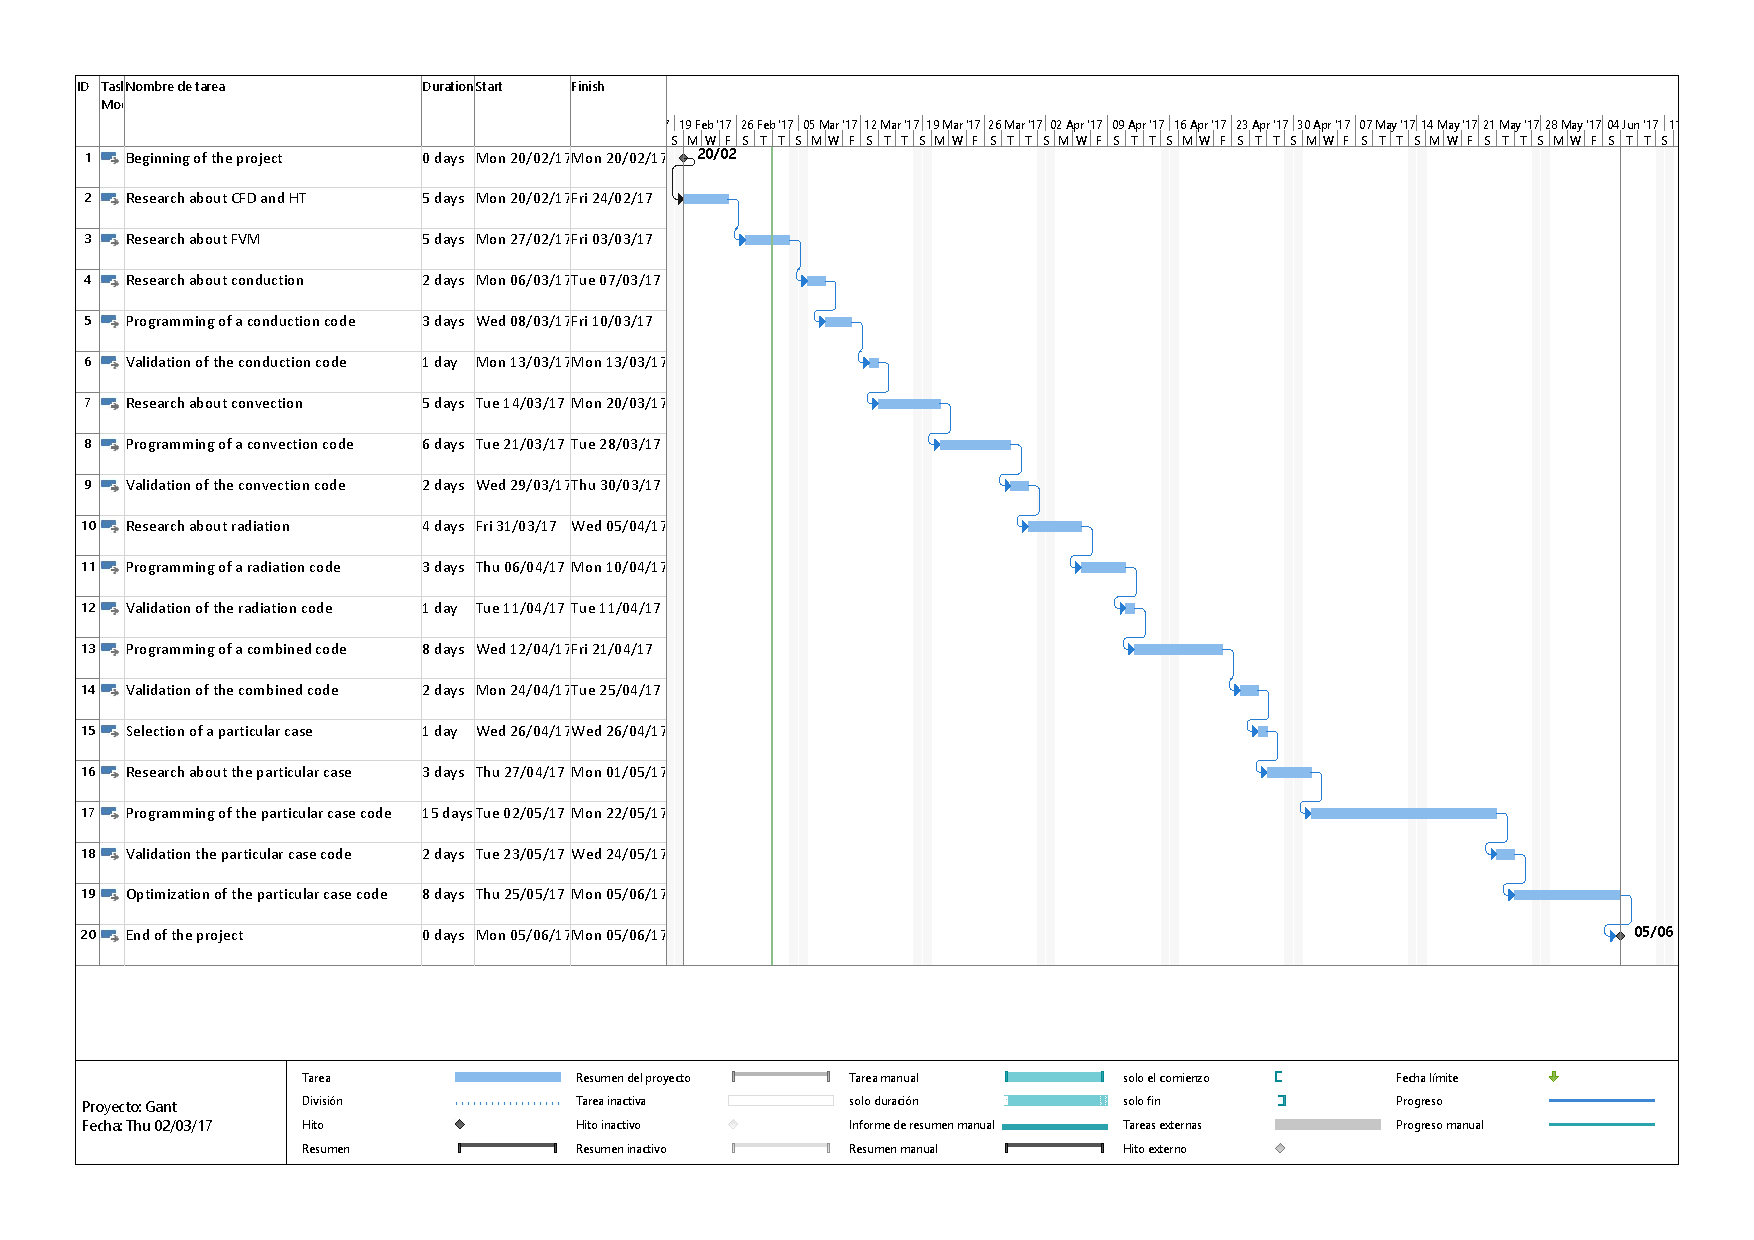
\includepdf[pages={1-}, landscape=true]{./Media/Gant.pdf}
\end{landscape}

\section{Bibliography}
\bibliographystyle{unsrt}
\bibliography{./Biblography}

\end{document}